\subsection{Fonctionnement des modules de l'application}
\label{section:eyrolles_modules}

Le \afm\ \asf\ oblige le développeur à construire son application web en la divisant sous forme de modules. Généralement, chaque module regroupe un ensemble de pages (nommées \emph{actions}) partageant un domaine fonctionnel commun. Cette bonne pratique favorise la maintenabilité et la lisibilité du code.

En effet, dans \aey, on compte une quarantaine de modules, comme \texttt{ey\-Referential\-Language} ou \texttt{eyContract}, gérant respectivement le ré\-fé\-ren\-ti\-el des langues et les contrats. Le module des contrats, par exemple, contient des pages comme celle listant les contrats ou encore celle permettant d'en créer.

Par rapport à ceux d'une application web lambda développée en \asf, les modules de l'\aintranet\ d'\aey\ ont la spécificité de se baser sur \asladmin\ et d'avoir subi une factorisation supplémentaire.


\subsubsection{Utilisation de \asladmin}

La plupart des vues du \alotdeux\ de l'\aintranet\ d'\aey\ sont générées grâce au \aplugin\ \asf\ \asladmin. Il a été développé en interne par \asl\ et est issu de l'abstraction du code d'un précédent projet. Il n'a rien à voir avec la fonctionnalité de génération d'administration intégrée à \asf. C'est encore un \aplugin\ très jeune : \aey\ est le premier projet qui l'utilise.

Le \aplugin\, tout comme la génération d'administration, permet de ne pas avoir à redévelopper la logique des opérations de base, telles que le listing d'éléments, sa pagination, son tri, ou encore la création, l'édition et la suppression d'éléments. Sa valeur ajoutée est qu'il apporte plus de flexibilité quant à la personnalisation de la logique et des différentes vues. Le tableau~\ref{table:eyrolles_sladmin_sladmin-vs-admin-gen} reprend une comparaison rapide des différences entre le moteur de génération d'administration de \asf\ et \asladmin.

\begin{table}
	\centering
	\begin{tabular}{|p{3cm}||p{4.5cm}|p{4.5cm}|}
		\hline
		& Génération d'administration & \asladmin\ \tabularnewline
		\hline
		\hline
		Format de configuration & \ayml & code \aphp \tabularnewline
		\hline
		Génération de code & oui & non \tabularnewline
		\hline
		Personnalisation de la logique & surcharge de code généré & surcharge d'actions de base \tabularnewline
		\hline
		Personnalisation des vues & surcharge de vues générées & écriture classique de vues \tabularnewline
		\hline
	\end{tabular}
	\caption{Comparaison entre la génération d'administration de \asf\ et \asladmin}
	\label{table:eyrolles_sladmin_sladmin-vs-admin-gen}
\end{table}

Ainsi, \asladmin\ permet de gagner du temps de développement et d'assurer une factorisation des opérations récurrentes d'administration du site.


\subsubsection{Agencement des modules}

Habituellement, les actions un module \asf\ reposent directement sur les classes d'actions de base intégrées au \afm. Ce comportement est nécessaire pour que les actions puissent d'exécuter et engendrer l'affichage des pages correspondantes.

L'utilisation de \asladmin\ change la donne : elle nécessite de baser les actions du module sur les classes d'actions propres au \aplugin, qui elles-mêmes se basent sur celles de \asf. Les classes d'actions de \asladmin\ intègrent les actions génériques décrites plus tôt, comme par exemple celles permettant de lister, créer ou supprimer des éléments.

La modélisation de l'\aintranet\ d'\aey\ est allée encore plus loin, en intégrant une nouvelle couche d'actions propres au projet entre celles des modules et celles de \asladmin. Son but est de permettre de modifier le comportement des actions de \asladmin\ afin qu'elles correspondent au mieux aux besoins du projet, sans pour autant avoir besoin de modifier le \aplugin.

Finalement, en plus d'être organisée horizontalement sous forme de modules, l'application est également découpée verticalement en différentes cou\-ches. Ses différentes fonctionnalités ont alors l'avantage de se distinguer les unes des autres, tout en partageant à la fois des bases communes. Cette organisation est illustrée dans la figure~\ref{figure:eyrolles_modules_couches}.

\begin{figure}
	\centering
	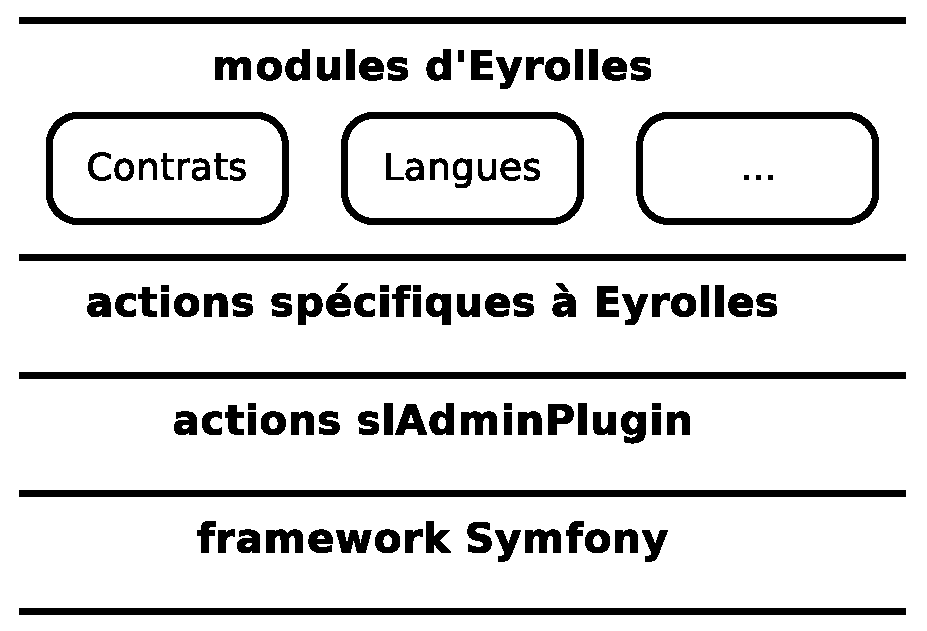
\includegraphics[scale=0.4]{eyrolles_modules_couches}
	\caption{Organisation des modules du \alotdeux\ d'\aey}
	\label{figure:eyrolles_modules_couches}
\end{figure}